%-------------------------------------------------------------------------------
%                            BAB II
%               TINJAUAN PUSTAKA DAN DASAR TEORI
%-------------------------------------------------------------------------------
\fancyhf{} 
\fancyfoot[C]{\thepage}
\chapter{TINJAUAN KEPUSTAKAAN}

\par Untuk mendukung penelitian ini, maka dalam bab ini akan dikemukakan beberapa rumusan teori pendukung yang dikutip dari berbagai referensi baik dalam bentuk buku, jurnal, maupun tulisan karya ilmiah yang memiliki kaitan dengan penelitian yang dibuat. 

\section{\textit{Speech Recognition}}
Kemampuan suatu komputer agar dapat mengenali apa yang diucapkan oleh seseorang berdasarkan sinyal suara yang diucapkan oleh seseorang disebut sebagai \textit{Automatic Speech Recognition} (ASR) \citep{azizah2015}. Selain untuk mengubah ucapan menjadi teks, ASR juga memiliki kemampuan untuk autentikasi \textit{biometric}, yaitu suatu kemampuan untuk mengenali pengguna dari suaranya. Hasil dari proses pengenalan dari suara seseorang dapat digunakan untuk melakukan tugas berdasarkan instruksi \citep{mustikarini2019}. Menjadi suatu kemudahan bagi manusia jika komputer dapat memahami apa yang diucapkan oleh manusia dan karena hal itu juga manusia dapat dengan mudah mengoperasikan komputer karena adanya teknologi yang disebut sebagai \textit{voice command} atau perintah suara \citep{widiyanto2015}.

\par Pada \textit{speech recognition}, sinyal suara akustik dipetakan oleh komputer ke beberapa bentuk makna abstrak dari ucapan tersebut. Suara harus dicocokkan dengan potongan suara yang disimpan sebelumnya, namun pada proses ini memiliki kesulitan yang tinggi jika \textit{sound bites} tidak cocok dengan potongan suara yang disimpan, sehingga analisis lebih lanjut harus dilakukan. Untuk mendapatkan kualitas \textit{speech recognition} yang lebih baik, berbagai metode ekstraksi fitur dan teknik pencocokan pola digunakan karena memiliki peran penting untuk memaksimalkan tingkat pengenalan suara dari berbagai orang \citep{saksamudre2015}.

\begin{figure}[H]
\centering
\shadowbox
{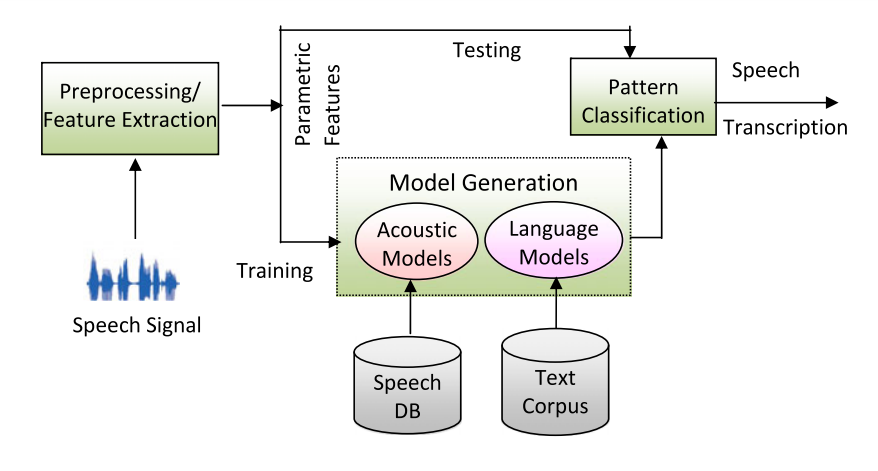
\includegraphics [width = 10cm, height= 5cm]{gambar/sr_arsitektur}}
\caption{Arsitektur ASR \citep{aggarwal2012}}.
\label{sr_arsitektur}
\end{figure}

\par Ada beberapa langkah atau tahapan yang digunakan untuk melakukan \textit{speech recognition} sesuai dengan gambar di atas, yaitu \textit{pre-processing/digital processing}, ekstraksi fitur, \textit{acoustic modelling}, \textit{language modelling} dan \textit{pattern classification/ decoding} \citep{aggarwal2012}. Pada pencocokan pola untuk \textit{speech recognition} memiliki 5 pendekatan, yaitu pendekatan berbasis \textit{template}, pendekatan berbasis pengetahuan, pendekatan berbasis jaringan saraf (\textit{neural network}), pendekatan berbasis \textit{Dynamic Time Warping} (DTW) dan pendekatan berbasis statistik \citep{saksamudre2015}.

\section{Ekstraksi Fitur}
Salah satu bagian penting dalam proses pengenalan ucapan adalah ekstraksi fitur. Dengan adanya ekstraksi fitur, mesin pengenalan ucapan dapat membedakan antara satu ucapan dengan ucapan lainnya \citep{gupta2016}. Ekstraksi fitur memiliki fungsi untuk menghapus informasi yang berlebihan dan tidak diinginkan dengan cara mendeteksi sekumpulan variabel dari sinyal suara yang dikorelasikan secara akustik, variabel tersebut disebut dengan fitur \citep{dua2018}. Ekstraksi fitur yang paling sering digunakan untuk pengolahan suara adalah Metode \textit{Mel-Frequency Cepstral Coefficients} (MFCC), karena metode tersebut dapat mempresentasikan sinyal dengan baik \citep{umar2019}.

\subsection{\textit{Mel Frequency Cepstral Coefficient} (MFCC)}
\par MFCC dapat berguna untuk mengoptimalkan sistem pengenalan suara dan menghasilkan hasil yang efisien, dengan dibangun suatu filter bank dari teknologi dan metode penelitian yang terus berubah. Dalam mengekstrak vektor fitur yang memiliki isi informasi tentang sinyal suara, MFCC menggunakan beberapa bagian dari produksi ucapan dan persepsi ucapan \citep{dua2018}. Berikut adalah langkah-langkah dan diagram alir pada ekstraksi fitur dengan MFCC:

\begin{figure}[H]
\centering
\shadowbox
{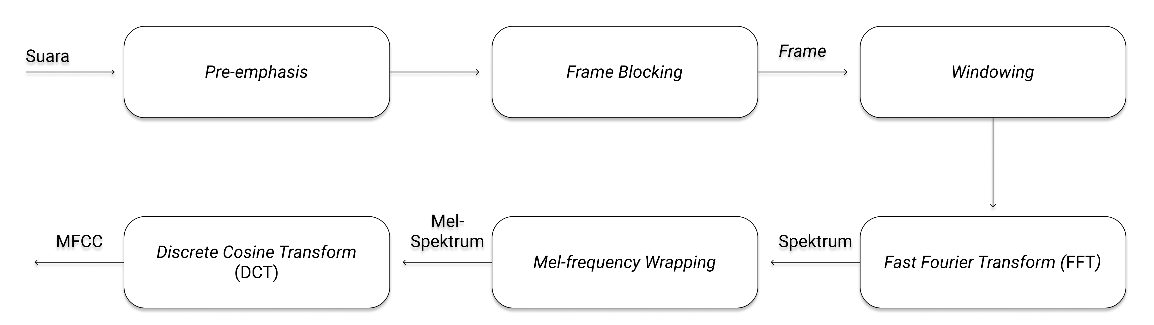
\includegraphics [width = 14cm, height= 5cm]{gambar/alir_mfcc}}
\caption{Diagram Alir \textit{Mel Frequency Cepstral Coefficient}}.
\label{alir_mfcc}
\end{figure}

\begin{enumerate}
\item \textit{Pre-emphasis}
\par Pada tahapan awal dalam menggunakan MFCC yaitu dengan \textit{pre-emphasis}. \textit{Pre-emphasis} dilakukan untuk mengurangi \textit{noise} karena sinyal suara yang didapat sering mengalami gangguan \textit{noise} \citep{heriyanto2018}. Dalam mengurangi efek samping saat mekanisme produksi suara, digunakanlah \textit{pre-emphasis} untuk menekan suara dengan frekuensi tinggi pada sinyal suara yang didapat. Fungsi lain \textit{pre-emphasis} dapat menguatkan puncak spektrum suara berfrekuensi tinggi \citep{efendi2019}. Secara matematis, \textit{pre-emphasis} dapat dirumuskan seperti pada persamaan berikut.

\begin{equation}
	y(n) = s(n) - as(n-1)
	\label{eqn1}
\end{equation}

\par Pada persamaan \ref{eqn1} dapat dijelaskan bahwa $y(n)$ adalah sinyal yang ditekan, $s(n)$ merupakan sinyal yang terdigitasi, serta $a$ adalah sebuah ketetapan filter \textit{pre-emhasis} atau sinyal yang diekstrak, dengan nilai 0.9 < $a$ < 1.0.

\item \textit{Frame blocking} dan \textit{Windowing}
\par Dalam menganalisis sinyal ucapan ke dalam bentuk \textit{frame} dibutuhkan tahap \textit{frame blocking} \citep{heriyanto2018}. Setelah sinyal ucapan melewati tahapan \textit{pre-emphasis} maka sinyal tersebut dibagi menjadi beberapa \textit{frame} dengan memuat N sampel sinyal pada masing-masing \textit{frame} dan \textit{frame} yang saling yang berdekatan akan dipisahkan sejauh M sampel \citep{laksono2018}. Setiap sampel dapat dibagi panjang \textit{frame} menjadi beberapa \textit{frame} berdasarkan waktu yang terletak di antara 20 ms hingga 40 ms \citep{laksono2018}. Di antara bagian-bagian \textit{frame} dengan \textit{frame} lainnya terdapat bagian yang bertumpang tindih atau yang disebut \textit{overlap}, hal ini berguna agar antar \textit{frame} saling berkesinambungan \citep{efendi2019}.

\par Untuk mencegah ketidaksinambungan sinyal suara dari ujung awal sampai ujung akhir dari proses \textit{frame blocking}, maka dilakukanlah \textit{windowing} \citep{efendi2019}. Tujuan dari \textit{windowing} adalah untuk mengurangi efek diskontinu pada ujung tiap \textit{frame} \citep{heriyanto2018}. Ada dua fungsi yang biasa digunakan yaitu \textit{Rectangular Window} dan \textit{Hamming Window} \citep{laksono2018}. Fungsi \textit{Rectangular Window} di tulis dalam persamaan \ref{eqn2} sebagai berikut.

\begin{equation}
	W = 
	\begin{cases}
		1 & 0 \le n \le N\\
		0 & L
	\end{cases}
	\label{eqn2}
\end{equation}

\par Fungsi di atas merupakan salah satu cara untuk menghindari diskontinu pada ujung \textit{window}, dengan cara meruncingkan sinyal menjadi nol atau dekat dengan nol, hal ini dapat mengurangi kesalahan yang terjadi \citep{laksono2018}. Lalu untuk Fungsi \textit{Hamming} sendiri dapat digambarkan seperti bentuk jendela dengan mempertimbangkan blok berikutnya di dalam rantai pemrosesan ekstraksi fitur serta menyatukan semua garis frekuensi yang terdekat \citep{laksono2018}. Fungsi \textit{Hamming} di tulis dalam persamaan \ref{eqn3} sebagai berikut.

\begin{equation}
	W(n) = 
	\begin{cases}
		0,54 - 0,46 \cos (\frac{2 \pi n}{N} - 1) & 0 \le n \le N-1\\
		0 & Otherwise
	\end{cases}
	\label{eqn3}
\end{equation}

\par Pada persamaan \ref{eqn3} dapat dijelaskan bahwa $W(n)$ merupakan \textit{Hamming Window}, jumlah dari sampel diinisialkan dengan $N$ dan $n$ menginisialkan pada sampel saat ini \citep{dua2018}. Lalu hasil persamaan \textit{Hamming Window} dikalikan dengan sinyal masukan/ \textit{innput} yang telah ditetapkan, perhitungan tersebut dapat dijelaskan pada persamaan \ref{eqn4} berikut ini \citep{laksono2018}.

\begin{equation}
	Y(n) = y(n) \times w(n)
	\label{eqn4}
\end{equation}

\par Pada persamaan \ref{eqn4} dapat dijelaskan bahwa $n$ merupakan banyaknya sampel tiap \textit{frame}, sinyal \textit{output} diwakilkan dengan $Y(n)$, sinyal \textit{input} diwakilkan dengan $y(n)$ dan $w(n)$ mewakilkan dari \textit{Hamming Window}.

\item \textit{Fast Fourier Transform} (FFT)
\par Untuk melakukan konversi sinyal dari domain waktu menjadi domain frekuensi dengan cepat digunakanlah \textit{Fast Fourier Transform} (FFT) \citep{efendi2019}. FFT berguna dalam mengubah konvolusi getaran celah suara dan respons yang didapat dari gelombang saluran suara dalam domain waktu \citep{laksono2018}. FFT sendiri dikembangkan karena suatu masalah dapat diselesaikan dengan mengubah atau memodelkan suatu permasalahan dalam representasi matematika dan mendapatkan keuntungan dalam segi efisiensi dibandingkan hal lainnya \citep{efendi2019}.

\item \textit{Mel-frequency Wrapping} 
\par Pada tahap ini spektrum yang dikeluarkan dari FFT di \textit{wrapping} sehingga menghasilkan \textit{mel-scale} agar resolusi frekuensi terhadap pendengaran manusia disesuaikan \citep{laksono2018}. Spektrum FFT memiliki nilai frekuensi yang sangat lebar, sehingga harus dipetakan ke dalam \textit{mel-scale} agar dapat mengetahui energi yang tersedia pada setiap titik dengan bantuan \textit{triangular} filter bank. Untuk mendapatkan batas-batas nilai tertinggi dan nilai terendah dari \textit{mel-scale} berdasarkan frekuensi suara dalam \textit{mel-frequency} pada setiap filter bank dihitung berdasarkan persamaan \ref{eqn5} berikut ini \citep{efendi2019}.

\begin{equation}
	mel = 2595 \log_{10} \Big(1 + \frac{f}{700}\Big)
	\label{eqn5}
\end{equation}

\par Pada persamaan \ref{eqn5} dapat dijelaskan bahwa $mel$ merupakan skala \textit{mel-frequency} dan frekuensi linear diwakilkan dengan $f$.

\item \textit{Discrete Cosine Transform} (DCT)
\par Tahap \textit{Discrete Cosine Transform} (DCT) digunakan untuk mengubah nilai koefisien \textit{mel-spectrum} menjadi ke domain waktu \citep{dua2018}.

\end{enumerate}

\section{\textit{Acoustic Model}}
\par Terdapat dua komponen utama pada sistem \textit{voice-to-text}, yang pertama adalah model akustik (\textit{acoustic model}) dan model bahasa (\textit{language model}). Model yang mengandung representasi statistik dari setiap suara yang berbeda dalam bentuk kata ataupun kalimat merupakan model akustik. Pada tiap-tiap representasi statistik tersebut dapat menentukan sebuah label yang disebut dengan suku kata (\textit{phonemes}) \citep{misbullah2020}. Model akustik memiliki dua tipe yang berbeda, yaitu \textit{phonemes} dan kata. Dua tipe tersebut diimplementasikan dengan berbagai metode seperti \textit{Hidden Markov Model} (HMM), \textit{Support Vector Machines} (SVM), \textit{Dynamic Bayesian Networks} (DBN) dan \textit{Artificial Neural Network} (ANN) \citep{gupta2016}. Sebagian besar sistem pengenalan suara saat ini menggunakan HMM untuk menangani variabilitas temporal ucapan lalu menggunakan \textit{Gaussian Mixture Models} (GMM) untuk menentukan seberapa baik status yang dihasilkan dari tiap HMM tersebut cocok dengan \textit{frame} atau \textit{short window of frames of coefficient} yang mewakili \textit{input} dari akustik \citep{hinton2012}. Cara alternatif yang terbaik untuk mengevaluasi kecocokan HMM dengan menggunakan \textit{Deep Neural Network} (DNN).

\subsection{\textit{Deep Neural Network} (DNN)}
\par DNN memiliki cara kerja dengan  mengambil beberapa koefisien dari frame sebagai masukannya dan menghasilkan keluaran berupa probabilitas posterior dari status HMM \citep{hinton2012}. \textit{Deep Neural Network} merupakan salah satu cabang dari \textit{machine learning} yang menggunakan konsep jaringan syaraf tiruan atau yang disebut dengan \textit{Neural Network} \citep{laksono2018}. DNN merupakan \textit{feed-forward}, \textit{feed-forward} itu sendiri adalah salah satu bagian di \textit{Artificial Neural Network} (ANN) yang memiliki lebih dari satu lapisan di \textit{hidden units} antara masukan atau keluarannya \citep{hinton2012}. Pada umumnya terdapat tiga struktur dari \textit{neural network}, yaitu \textit{input layer}, \textit{hidden layer} dan \textit{output layer}. Pada \textit{input layer} tiap \textit{node} merepresentasikan vektor untuk jumlah data \textit{input}, lalu pada \textit{hidden layer} memiliki fungsi untuk mengontrol apakah informasi dapat diketahui atau tidak dari \textit{input layer} yang akan diteruskan ke layer berikutnya dan yang terakhir setiap \textit{node} pada \textit{output layer} didefinisikan sebagai target dari kelas yang akan diprediksi \citep{misbullah2020}. DNN terbukti dapat mengungguli GMM dalam berbagai tolak ukur pengenalan ucapan serta terkadang dengan margin yang besar, karena DNN sendiri memiliki banyak \textit{hidden layer} dan dibuktikan dengan dilatih menggunakan metode baru \citep{hinton2012}. Penggambaran model umum dari DNN ditunjukkan seperti pada Gambar \ref{dnn_arsitektur}, di mana variasi proses, jumlah dan urutan \textit{hidden layer} tergantung pada arsitekturnya \citep{musiol2016}. 

\begin{figure}[H]
\centering
\shadowbox
{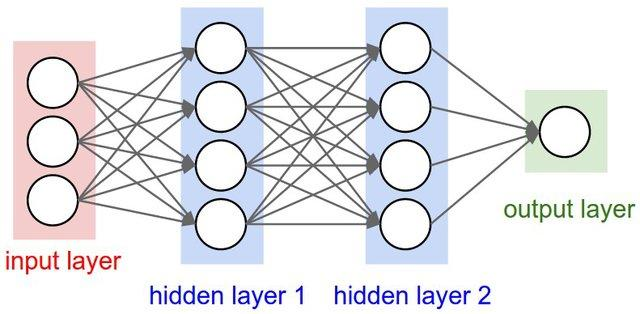
\includegraphics [width = 10cm, height= 5cm]{gambar/dnn_arsitektur}}
\caption{Model Umum dari \textit{Deep Neural Network} \citep{musiol2016}}.
\label{dnn_arsitektur}
\end{figure}

\par \textit{Neural Network} sendiri memiliki dua arsitektur, yaitu \textit{single layer perseptron} dan \textit{multi layer perseptron}. \textit{Single layer persepton} mempunyai satu \textit{hidden layer} yang digunakan, lalu pada \textit{multi layer perseptron} mempunyai lebih dari dua \textit{hidden layer} yang digunakan \citep{laksono2018}. Untuk mendapatkan hasil yang akurat, pada \textit{Deep Neural Network} atau \textit{Deep Learning} menggunakan jumlah \textit{hidden layer} yang sangat banyak \citep{laksono2018}.

\section{Kaldi \textit{Toolkit}}
Salah satu \textit{toolkit} untuk pengenalan suara yang \textit{open-source} adalah Kaldi, Kaldi sendiri ditulis dalam bahasa C++ dan di bawah lisensi Apache v2.0 \citep{povey2011}. Kaldi bergantung dengan dua \textit{library} dari luar yang tersedia secara bebas, \textit{library} yang pertama adalah OpenFst digunakan untuk \textit{finite-state framework} lalu untuk \textit{library} aljabar linear ekstensif menggunakan "\textit{Basic Linear Algebra Subrutin}" (BLAS) dan "\textit{Linear Algebra PACKage}" (LAPACK) \citep{povey2011}. Fitur pada Kaldi yang dapat digunakan adalah ekstraksi fitur yang paling umum digunakan, pemodelan akustik dengan beberapa model umum namun dapat diperluas dengan model jenis baru, \textit{phonetic decision tree} yang efisien untuk ukuran konteks arbitrer dan juga mendukung dengan berbagai pendekatan, pemodelan bahasa dapat menggunakan model bahasa apa pun yang dapat direpresentasikan sebagai \textit{finite-state transducer} (FST) serta dapat menggunakan \textit{toolkit} IRSTLM untuk membangun pemodelan Bahasa dari teks mentah, dan dapat membuat grafik decoding yang didasarkan pada \textit{Weighted Finite State Transducers} (WFSTs) \citep{povey2011}. Kaldi terus dikembangkan dan sedang mengerjakan model Bahasa yang besar dalam kerangka FST, pembuatan kisi dan pelatihan diskriminatif \citep{povey2011}.

\section{\textit{Indoor Positioning System}}
\textit{Indoor Positioning System} (IPS) dapat menemukan lokasi orang atau objek di dalam ruangan dengan menggunakan gelombang radio, medan magnet, sinyal akustik serta informasi sensoris yang dikumpulkan oleh alat teknologi berupa \textit{smartphone}, tablet, atau perangkat pintar lainnya \citep{atlas2016}. IPS memiliki beberapa pendekatan yaitu, \textit{positioning systems} berbasis WiFi (WPS), \textit{positioning systems} berbasis \textit{Bluetooth Low Energy} (BLE), sistem berbasis Identifikasi Frekuensi Radio (RFID) dan teknologi \textit{Ultra-Wide Band} (UWB) atau \textit{Visible Light Communication} (VLC) \citep{canton2017}.

\par \textit{Bluetooth Low Energy} (BLE) \textit{Beacon} merupakan suatu perangkat yang berukuran kecil dan menggunakan baterai sebagai sumber tenaganya, BLE dapat mengirimkan sinyal di area yang terbatas sampai 20 meter / 70 kaki dan bereaksi terhadap lokasi seseorang yang berada dalam jangkauan \citep{atlas2016}. BLE memiliki kelebihan yang dapat mengalahkan WPS yang telah popular dimasa lalu. BLE menawarkan harga yang lebih murah dan memiliki daya yang rendah, sehingga untuk infrastruktur yang tidak memungkinkan adanya WiFi dapat menjadi pilihan terbaik \citep{canton2017}. BLE dikenal sebagai pilihan yang terbaik karena mampu menyiarkan data menggunakan daya yang minimal hal itu didasarkan karena teknologi \textit{Bluetooth} yang digunakannya, serta BLE ideal untuk perangkat yang dapat berfungsi tanpa gangguan untuk jangka waktu yang lama karena menggunakan baterai kecil. Dari hal yang sudah dijelaskan sebelumnya BLE dapat berfungsi dengan baik untuk keperluan navigasi di dalam ruangan \citep{herrera2016}. 


%-----------------------------------------------------------------------------%

% Baris ini digunakan untuk membantu dalam melakukan sitasi
% Karena diapit dengan comment, maka baris ini akan diabaikan
% oleh compiler LaTeX.
\begin{comment}
\bibliography{daftar-pustaka}
\end{comment}
